\documentclass[aspectratio=1610]{beamer}
\hypersetup{
        unicode=true,
        linkcolor=blue,
        anchorcolor=blue,
        citecolor=green,
        filecolor=black,
        urlcolor=blue
    }

%%%%% PACKAGES HERE
%% \usepackage{}
\usepackage{amsmath}
\usepackage{amssymb}
\usepackage{listings}
\usepackage{textcomp}
% \usepackage{minted}
\usepackage[backend=bibtex]{biblatex}
%\usepackage[style=authortitle,backend=biber]{biblatex}
\addbibresource{references.bib}

%%%%%%%%%%%%%%%%%%%%%%%%%%%%%%%%%%%
%% DO NOT CHANGE

\usetheme{default}
\useinnertheme{circles}
\useoutertheme{infolines}
\usefonttheme{serif}

\usepackage{etoolbox}

%% T for navigation symbols
%%\setbeamertemplate{navigation symbols}{}

%% T for header
%% \setbeamertemplate{headline}{%
%%   \leavevmode%
%%   \ifdefempty{\insertsubsectionhead}{
%%     \begin{beamercolorbox}[wd=0.99\paperwidth,ht=2.25ex,dp=1ex,center]{section in head/foot}%
%%       % \hbox to .5\paperwidth{\hfil\insertsectionhead\hfil}
%%       \insertsectionhead
%%     \end{beamercolorbox}%
%%   }{
%%     \begin{beamercolorbox}[wd=.44\paperwidth,ht=2.25ex,dp=1ex,right]{section in head/foot}%
%%       % \hbox to .5\paperwidth{\hfil\insertsectionhead\hfil}
%%       \insertsectionhead
%%     \end{beamercolorbox}%
%%     \begin{beamercolorbox}[wd=.1\paperwidth,ht=2.25ex,dp=1ex,center]{section in head/foot}%
%%       % \hbox to .5\paperwidth{\hfil\insertsectionhead\hfil}
%%       -
%%     \end{beamercolorbox}%
%%     \begin{beamercolorbox}[wd=.44\paperwidth,ht=2.25ex,dp=1ex,left]{subsection in head/foot}%
%%       % \hbox to .5\paperwidth{\hfil\insertsubsectionhead\hfil}
%%       \insertsubsectionhead
%%     \end{beamercolorbox}
%%   }%
%% }

%% T for frame title
\setbeamertemplate{frametitle}{%
  \usebeamerfont{frametitle}\insertframetitle\strut%
  \vskip-0\baselineskip%
  \leaders\vrule width .95\paperwidth\vskip1pt%
  \vskip0pt%
  \nointerlineskip
}

%% T for footer
\setbeamercolor{footlinecolor}{fg=cyan,bg=green}
\setbeamercolor{author in head/foot}{fg=blue}

\setbeamertemplate{footline}{%
  \leavevmode%
  \hbox{%
  \begin{beamercolorbox}[wd=.26\paperwidth,ht=2.25ex,dp=1ex,left]{author in head/foot}%
    \hspace*{2ex}\usebeamerfont{author in head/foot} Dept. CSE, UT Arlington
  \end{beamercolorbox}%
  \begin{beamercolorbox}[wd=.50\paperwidth,ht=2.25ex,dp=1ex,center]{author in head/foot}%
    \usebeamerfont{title in head/foot}Scalable Modeling \& Imaging \& Learning Lab (SMILE)
  \end{beamercolorbox}%
  \begin{beamercolorbox}[wd=.24\paperwidth,ht=2.25ex,dp=1ex,right]{date in head/foot}%
    \usebeamerfont{date in head/foot}
    \insertshortdate{}\hspace*{1em}  % date
    \insertframenumber/\inserttotalframenumber\hspace*{2ex}
  \end{beamercolorbox}}%
  \vskip0pt%
}
%%%%%%%%%%%%%%%%%%%%%%%%%%%%%%%%%%%%%%%%%%%%%%%%

%% Start from here.
\title{A collection of modular open source C++ libraries for the development of logic synthesis applications\\ By EFPL}
\author{Gcc}
\date\today

\begin{document}

\begin{frame}[plain]
  \titlepage
  %  Title page
\end{frame}
\section{induction}
\begin{frame}
  SIS, 
\end{frame}

\section{example}
\begin{frame}{problem}
  \begin{figure}[htbq]
    \centering
    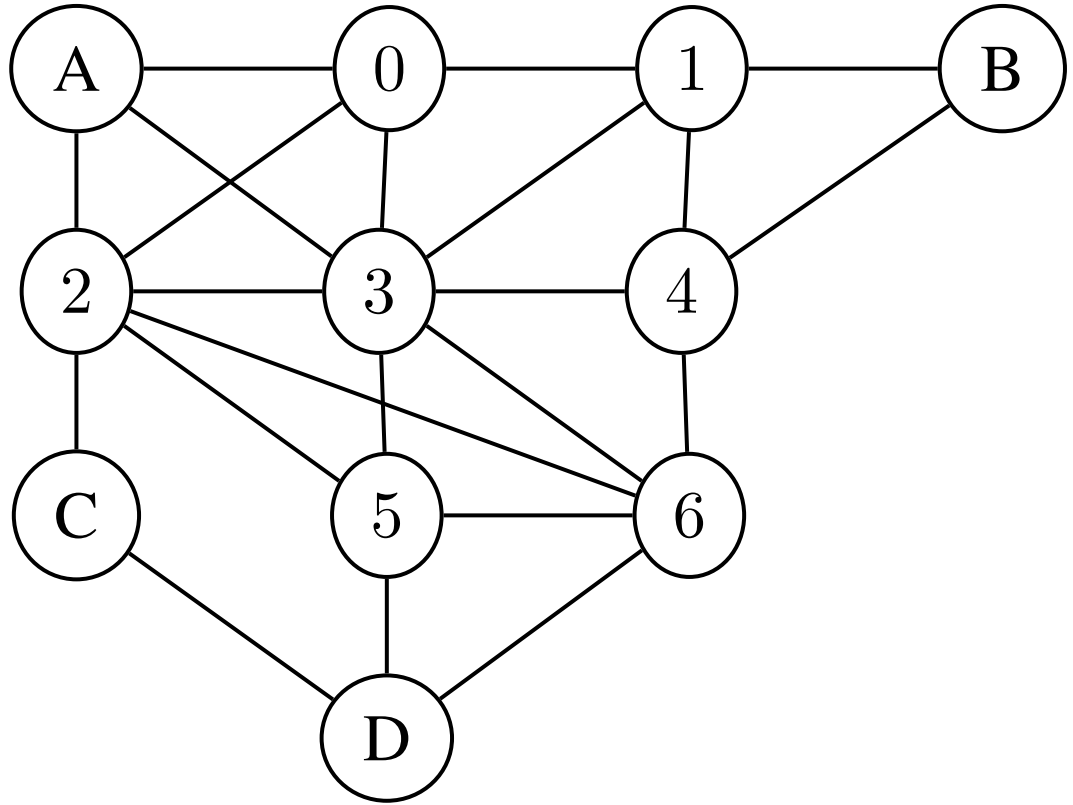
\includegraphics[width=0.5\textwidth]{problem.png}
    \caption{Zed city as an undirected graph} 
    \label{fig-zed}
  \end{figure}
\end{frame}
\begin{frame}{boolean function}
  \begin{columns}
    \begin{column}{0.45}
      a
    \end{column}
    \begin{column}{0.45}
      a
    \end{column}
  \end{columns}
\end{frame}
\begin{frame}{boolean function}
  code here
\end{frame}
\begin{frame}{flow}
  \begin{itemize}
    \item Angel:
    \item Tweedledum:
    \item Caterpillar:
  \end{itemize}
\end{frame}
\begin{frame}{initial state}
  \begin{itemize}
    \item formality\footcite{}
  \end{itemize}
\end{frame}
\begin{frame}{compiling oracle}
  \begin{itemize}
    \item 
  \end{itemize}
\end{frame}
\begin{frame}{XAG}
  \begin{itemize}
    \item change a for b
    \item figure
  \end{itemize}
\end{frame}
\begin{frame}{XAG example}
  \begin{itemize}
    \item for
    \item we 
  \end{itemize}
\end{frame}
\begin{frame}{result}
  table   
\end{frame}

\section{tweedledum}
\begin{frame}{induction}  
  ABC 
\end{frame}
\begin{frame}{compilation flow}
  \begin{figure}[htbq]
    \centering
    \includegraphics[width=0.8\textwidth]{Snipaste_2022-10-18_11-09-36.png}
    \caption{compilation flow overview} 
    \label{fig-compilation}
  \end{figure}
\end{frame}
\begin{frame}{flexibility}
  \begin{figure}[htbq]
    \centering
    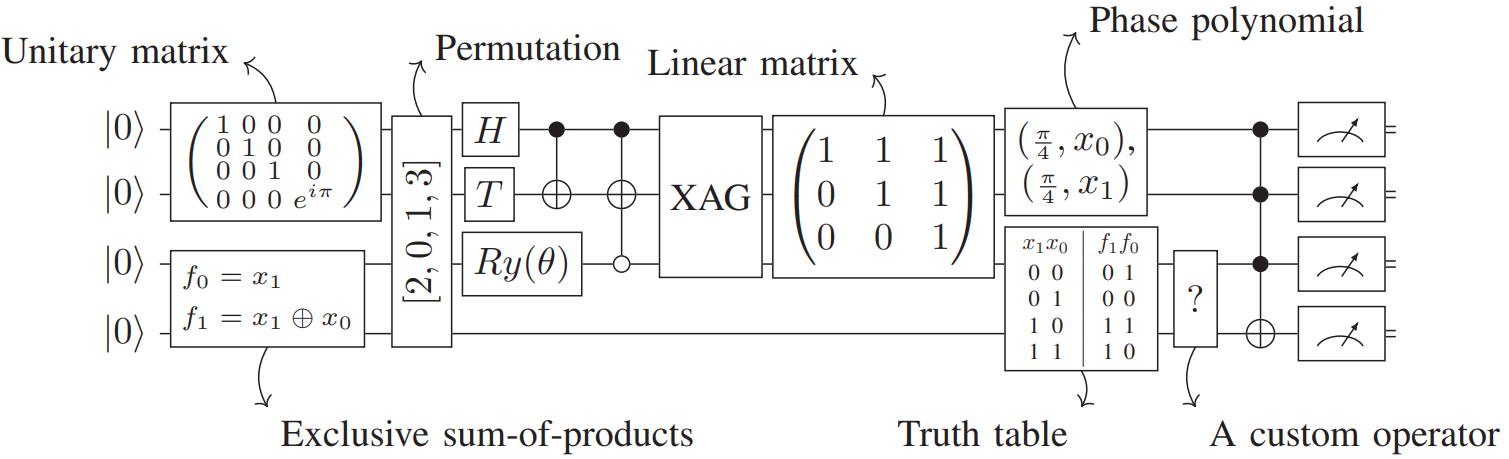
\includegraphics[width=0.9\textwidth]{flex.png}
    \caption{tweedledum's IR flexibility} 
    \label{fig-flex}
  \end{figure}
\end{frame}
\begin{frame}{synthesis}
  \begin{itemize}
    \item 
  \end{itemize}  
\end{frame}
\begin{frame}{synthesis}
  \begin{figure}[htbq]
    \centering
    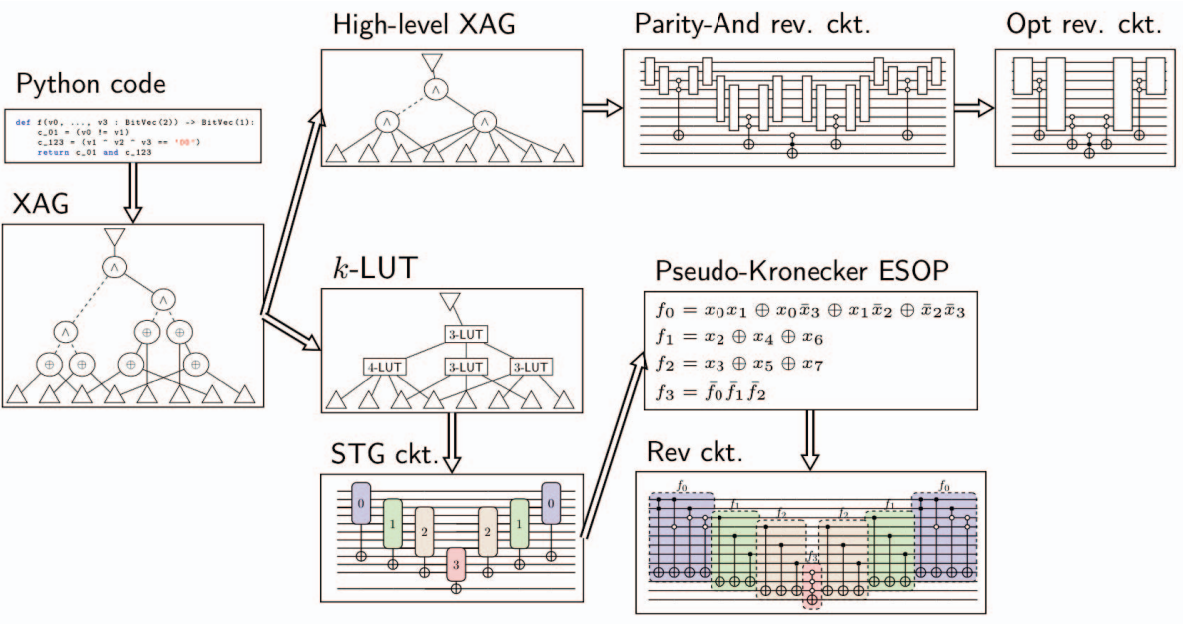
\includegraphics[width=0.7\textwidth]{boolean.png}
    \caption{overview of possible Boolean function synthesis flows} 
    \label{fig-boolean}
  \end{figure}
\end{frame}
\begin{frame}{compilation passes}
  \begin{itemize}
    \item 
  \end{itemize}
\end{frame}
\section*{}
\begin{frame}[noframenumbering,allowframebreaks,t]
	\frametitle{references}
	\printbibliography
\end{frame}
\begin{frame}
\centering
\Huge{END\\Thank you}
\end{frame}
\end{document}